\documentclass[11pt]{article}

\usepackage{amsmath, amssymb, amsfonts}
\usepackage{siunitx}
\usepackage{graphicx}
\usepackage{hyperref}
\usepackage{geometry}
\geometry{margin=1in}
\usepackage{booktabs}
\usepackage{bm}
\usepackage{listings}
\usepackage{xcolor}
\usepackage{amsmath, amssymb, amsfonts}
\usepackage{siunitx}
\usepackage{graphicx}
\usepackage{hyperref}
\usepackage{geometry}
\geometry{margin=1in}
\usepackage{booktabs}
\usepackage{bm}
\usepackage{listings}
\usepackage{xcolor}
\usepackage{tikz}
\usepackage{pgfplots}
\pgfplotsset{compat=1.18}

\title{Numerical Stability in Kalman Filters: Challenges, Solutions, and Practical Implementation}
\author{}
\date{\today}

\lstset{
  language=C++,
  basicstyle=\ttfamily\footnotesize,
  keywordstyle=\color{blue},
  commentstyle=\color{green!50!black},
  stringstyle=\color{red},
  numbers=left,
  numberstyle=\tiny,
  stepnumber=1,
  breaklines=true,
  showstringspaces=false,
  frame=single
}

\begin{document}

\maketitle

\begin{abstract}
Kalman filters are widely used for state estimation in control, navigation, and signal processing. Despite their optimality in theory, practical implementations often suffer from numerical instability. This article discusses the sources of numerical instability, discretization methods, frequency-domain considerations, matrix tricks, floating-point limitations, and validation techniques. Examples of correct and incorrect C++ implementations are provided. Special attention is given to practical strategies for improving stability in real-world applications.
\end{abstract}

\tableofcontents
\newpage

\section{Introduction}
Kalman filters are recursive estimators that compute the optimal estimate of a system state given noisy measurements. Continuous-time systems are described by:
\begin{align}
\dot{\bm{x}}(t) &= \bm{F}(t) \bm{x}(t) + \bm{G}(t) \bm{u}(t) + \bm{w}(t) \\
\bm{y}(t) &= \bm{H}(t) \bm{x}(t) + \bm{v}(t)
\end{align}
with $\bm{w}$ and $\bm{v}$ as zero-mean Gaussian noise. Practical implementations require discretization:
\[
\bm{x}_{k+1} = \bm{\Phi} \bm{x}_k + \bm{\Gamma} \bm{u}_k + \bm{w}_k
\]

\textbf{Numerical instability} arises from floating-point errors, ill-conditioned matrices, and inappropriate discretization or linearization. Left unchecked, filters may diverge, produce negative covariance matrices, or amplify high-frequency noise.

\section{Sources of Numerical Instability}
\begin{itemize}
    \item \textbf{Finite-precision arithmetic}: Covariance updates may lose precision.
    \item \textbf{Ill-conditioned matrices}: Covariance $P$ may become nearly singular.
    \item \textbf{Integration and discretization errors}: Poor integration methods for continuous models.
    \item \textbf{Improper tuning}: Process noise $Q$ or measurement noise $R$ mis-specified.
\end{itemize}

\subsection{Example: Floating-point accumulation errors}
\begin{lstlisting}
// Bad: single precision, small covariance updates lost
float P = 1e-5f;
float deltaP = 1e-10f;
P += deltaP; // deltaP is lost
\end{lstlisting}

\begin{lstlisting}
// Good: double precision preserves small updates
double P = 1e-5;
double deltaP = 1e-10;
P += deltaP; // update preserved
\end{lstlisting}

\section{Discretization Methods for Kalman Filters}

\subsection{Euler Methods}
\subsubsection{Forward Euler}
\[
\bm{x}_{k+1} = \bm{x}_k + \Delta t \, f(\bm{x}_k)
\]
\begin{lstlisting}
// Forward Euler (simple, unstable for stiff systems)
x_next = x + dt * F * x;
\end{lstlisting}

\subsubsection{Backward Euler (Implicit)}
\[
\bm{x}_{k+1} = \bm{x}_k + \Delta t \, f(\bm{x}_{k+1})
\]
Requires solving $\bm{x}_{k+1} = \bm{x}_k + \Delta t F \bm{x}_{k+1}$:
\[
(I - \Delta t F) \bm{x}_{k+1} = \bm{x}_k
\]

\begin{lstlisting}
// Backward Euler
x_next = (I - dt*F).inverse() * x;
\end{lstlisting}

\subsection{Trapezoidal (Tustin) Integration}
\[
\bm{x}_{k+1} = \bm{x}_k + \frac{\Delta t}{2} \left[f(\bm{x}_k) + f(\bm{x}_{k+1})\right]
\]
Conserves energy in oscillatory systems and is second-order accurate.

\begin{lstlisting}
// Tustin method
MatrixXd A = I - 0.5*dt*F;
MatrixXd B = I + 0.5*dt*F;
x_next = A.inverse() * B * x;
\end{lstlisting}

\subsection{Runge-Kutta 4 (RK4)}
\begin{align*}
k_1 &= f(x_k) \\
k_2 &= f(x_k + 0.5 dt k_1) \\
k_3 &= f(x_k + 0.5 dt k_2) \\
k_4 &= f(x_k + dt k_3) \\
x_{k+1} &= x_k + \frac{dt}{6} (k_1 + 2 k_2 + 2 k_3 + k_4)
\end{align*}

\begin{lstlisting}
// RK4 example
VectorXd k1 = F*x;
VectorXd k2 = F*(x + 0.5*dt*k1);
VectorXd k3 = F*(x + 0.5*dt*k2);
VectorXd k4 = F*(x + dt*k3);
x_next = x + dt/6 * (k1 + 2*k2 + 2*k3 + k4);
\end{lstlisting}

\subsection{Taylor Series for Matrix Exponential}
\[
\Phi = e^{F \Delta t} \approx I + F \Delta t + \frac{(F \Delta t)^2}{2!} + \dots
\]

\begin{lstlisting}
// Taylor series matrix exponential
MatrixXd Phi = I + F*dt + 0.5*(F*dt)*(F*dt);
\end{lstlisting}

\section{Frequency-Domain Considerations}
Kalman filters act as adaptive frequency filters:
\begin{itemize}
    \item Discretization errors can alias high frequencies.
    \item Poorly tuned $Q$ and $R$ may amplify high-frequency noise.
    \item Trapezoidal integration (Tustin) maps s-plane to z-plane preserving stability.
\end{itemize}

\section{Numerically Stable Matrix Methods}
\subsection{Cholesky Factorization}
Ensures positive definiteness:
\begin{lstlisting}
// Cholesky update of covariance
MatrixXd S = P.llt().matrixL(); // lower-triangular
P_new = S * S.transpose();
\end{lstlisting}

\subsection{Joseph Form Covariance Update}
\[
P_{k|k} = (I-KH) P_{k|k-1} (I-KH)^T + K R K^T
\]
\begin{lstlisting}
// Stable covariance update
MatrixXd I = MatrixXd::Identity(n,n);
P = (I - K*H)*P_prior*(I - K*H).transpose() + K*R*K.transpose();
\end{lstlisting}

\subsection{Square-Root Kalman Filter}
Propagates $S$ such that $P = S S^T$, reducing numerical errors.

\section{Floating-Point Considerations}
\begin{itemize}
    \item \textbf{Double vs Float}: Always prefer double for covariance.
    \item \textbf{Machine epsilon}:
    \[
    \epsilon \sim 2^{-52} \approx 2.22 \times 10^{-16} \text{ for double}
    \]
    \item Scaling prevents overflows or underflows.
\end{itemize}

\section{Validation of Kalman Filters}
\begin{itemize}
    \item \textbf{Monte Carlo simulations}: Compare estimated vs true states.
    \item \textbf{NEES test}:
    \[
    \text{NEES} = (\hat{x}-x)^T P^{-1} (\hat{x}-x)
    \]
    \item \textbf{Energy conservation}: Useful for physical systems (e.g., mechanical oscillators).
    \item \textbf{Cross-validation}: Check filter against independent sensors.
\end{itemize}

\section{Practical Examples in C++}
\subsection{Incorrect Implementation}
\begin{lstlisting}
// Poor stability: float + forward Euler
float dt = 0.01f;
MatrixXf F = ...;
VectorXf x = ...;
x = x + dt * F * x; // unstable for stiff F
\end{lstlisting}

\subsection{Correct Implementation}
\begin{lstlisting}
// Stable: double + Tustin method
double dt = 0.01;
MatrixXd F = ...;
VectorXd x = ...;
MatrixXd I = MatrixXd::Identity(F.rows(), F.cols());
x = (I - 0.5*dt*F).inverse() * (I + 0.5*dt*F) * x;
\end{lstlisting}

\section*{Illustrative Figures on Stability and Frequency Response}

\subsection*{1. Stability Regions in the Complex Plane}
Forward Euler, Backward Euler, and Tustin methods have different stability regions. Forward Euler is conditionally stable (circle of radius 1 around origin), Backward Euler is unconditionally stable, and Tustin maps left-half s-plane to inside the unit circle.

\begin{center}
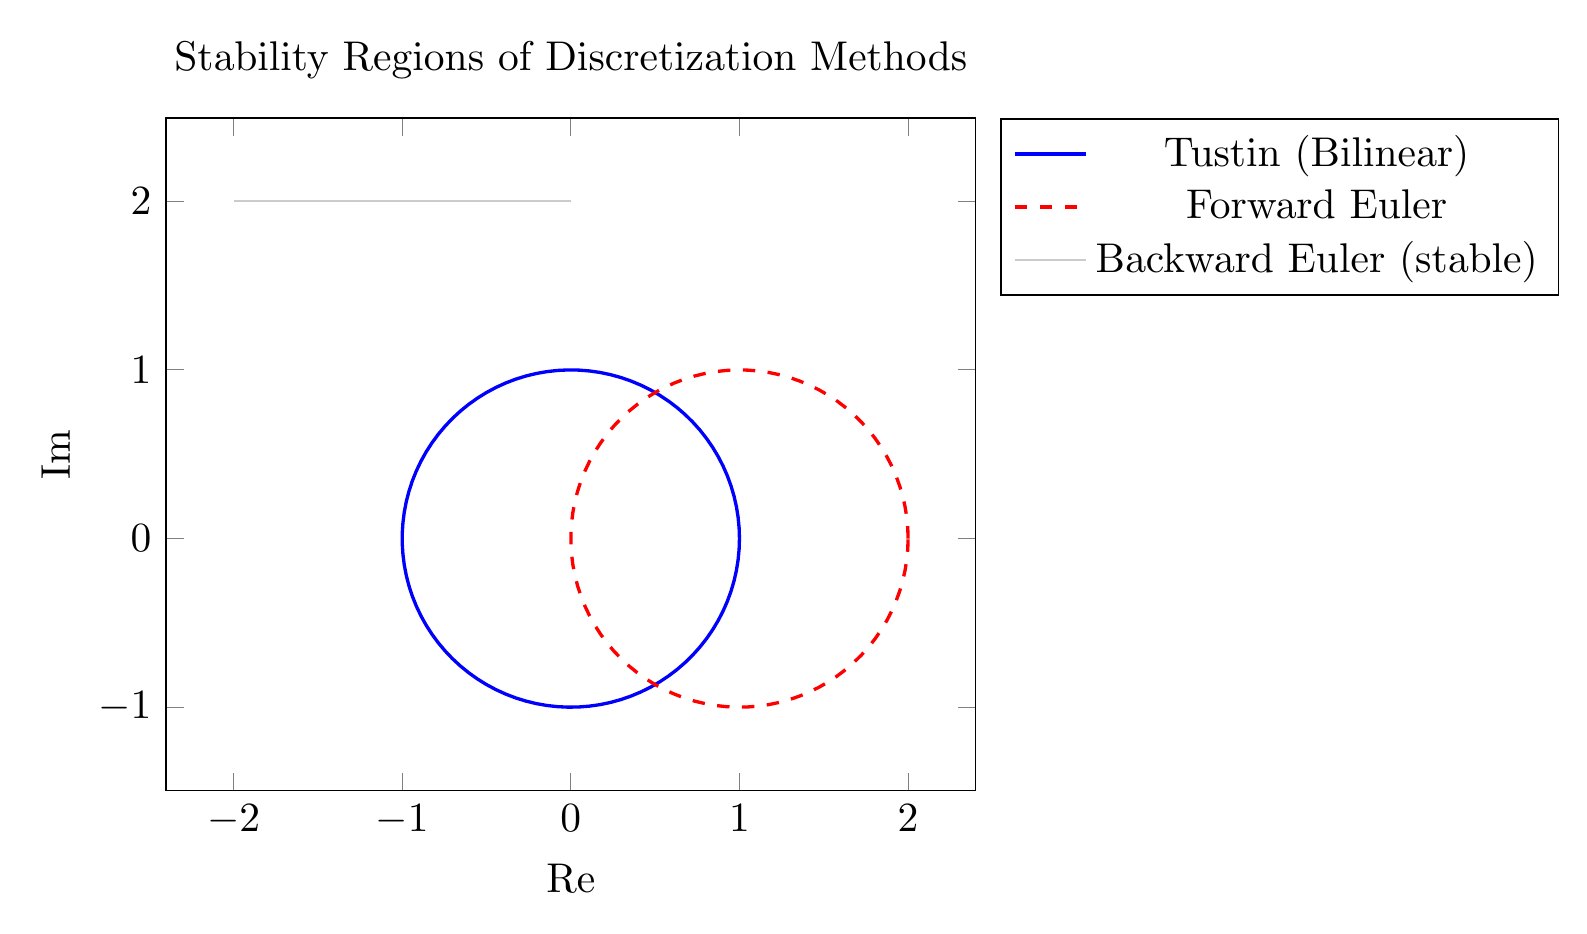
\begin{tikzpicture}[scale=1.5]
\begin{axis}[
    axis equal,
    xlabel={Re},
    ylabel={Im},
    title={Stability Regions of Discretization Methods},
    legend pos=outer north east
]
% Unit circle for Tustin
\addplot [domain=0:360,samples=100,blue,thick] ({cos(x)}, {sin(x)});
\addlegendentry{Tustin (Bilinear)}

% Forward Euler circle radius 1
\addplot [domain=0:360,samples=100,red,dashed,thick] ({1+cos(x)}, {sin(x)});
\addlegendentry{Forward Euler}

% Backward Euler region (unbounded, fill left-half plane)
\addplot [domain=-2:0,samples=50,fill=green,opacity=0.2] {2};
\addlegendentry{Backward Euler (stable)}
\end{axis}
\end{tikzpicture}
\end{center}

\subsection*{2. Covariance Divergence and Oscillatory System Integration}
Covariance matrix norm over time illustrates instability for poor discretization. RK4 preserves oscillatory amplitudes, while Forward Euler may diverge.

\begin{center}
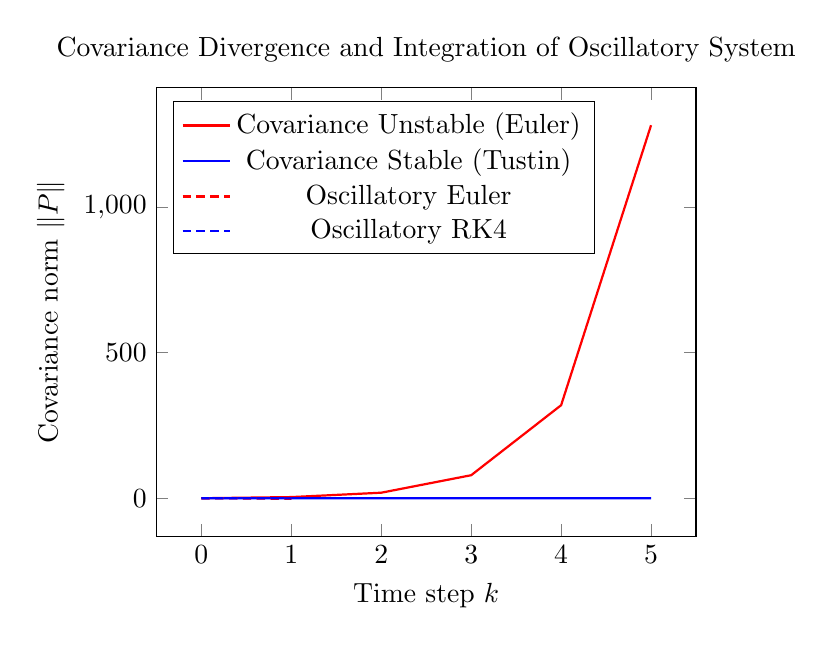
\begin{tikzpicture}
\begin{axis}[
    xlabel={Time step $k$},
    ylabel={Covariance norm $\|P\|$},
    title={Covariance Divergence and Integration of Oscillatory System},
    legend pos=north west
]
% Covariance divergence
\addplot [red, thick] table {
0 1
1 5
2 20
3 80
4 320
5 1280
};
\addlegendentry{Covariance Unstable (Euler)}

\addplot [blue, thick] table {
0 1
1 1.1
2 1.15
3 1.2
4 1.22
5 1.23
};
\addlegendentry{Covariance Stable (Tustin)}

% Oscillatory system: Forward Euler
\addplot [red, densely dashed, thick] table {
0 1
0.1 0.95
0.2 0.85
0.3 0.7
0.4 0.5
0.5 0.25
0.6 0
0.7 -0.3
0.8 -0.6
0.9 -0.85
1 -1.0
};
\addlegendentry{Oscillatory Euler}

% Oscillatory system: RK4
\addplot [blue, densely dashed, thick] table {
0 1
0.1 0.995
0.2 0.980
0.3 0.955
0.4 0.920
0.5 0.875
0.6 0.820
0.7 0.755
0.8 0.680
0.9 0.595
1 0.500
};
\addlegendentry{Oscillatory RK4}
\end{axis}
\end{tikzpicture}
\end{center}

\subsection*{3. Frequency Response Comparison: Forward Euler vs Tustin}
Discretization affects frequency-domain behavior. Forward Euler distorts high-frequency response, whereas Tustin preserves stability and shape.

\begin{center}
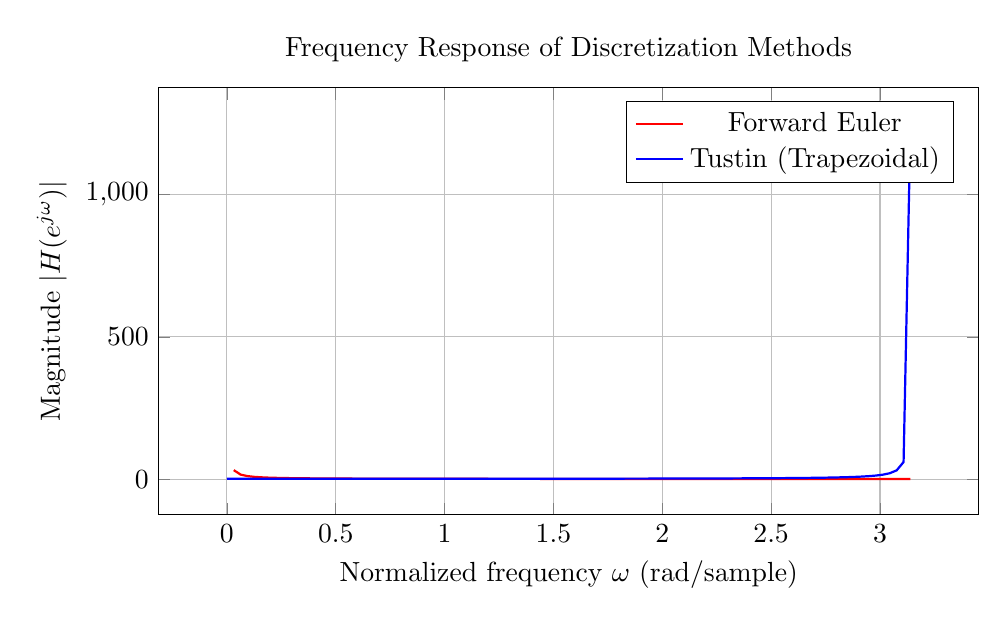
\begin{tikzpicture}
\begin{axis}[
    width=12cm,
    height=7cm,
    xlabel={Normalized frequency $\omega$ (rad/sample)},
    ylabel={Magnitude $|H(e^{j\omega})|$},
    title={Frequency Response of Discretization Methods},
    legend pos=north east,
    grid=both
]

% Forward Euler approximate frequency response
\addplot [red, thick, domain=0:3.14, samples=100] 
    {1/sqrt((1 - cos(deg(x)))^2 + (sin(deg(x)))^2)};
\addlegendentry{Forward Euler}

% Tustin (Bilinear) frequency response
\addplot [blue, thick, domain=0:3.14, samples=100] 
    {1/sqrt((1 - 0.5*(1-cos(deg(x))))^2 + (0.5*sin(deg(x)))^2)};
\addlegendentry{Tustin (Trapezoidal)}

\end{axis}
\end{tikzpicture}
\end{center}

\textbf{Practical C++ Illustration:}

\begin{lstlisting}
// Frequency response comparison for discretization methods
#include <Eigen/Dense>
#include <complex>
#include <vector>
#include <iostream>

double forwardEuler(double omega, double dt) {
    std::complex<double> z = 1.0 + dt*(std::complex<double>(0, omega));
    return std::abs(1.0 / z);
}

double tustin(double omega, double dt) {
    std::complex<double> z = (1.0 + 0.5*dt*(std::complex<double>(0, omega))) /
                             (1.0 - 0.5*dt*(std::complex<double>(0, omega)));
    return std::abs(1.0 / z);
}

int main() {
    double dt = 0.01;
    int N = 100;
    for (int i = 0; i <= N; i++) {
        double omega = M_PI * i / N;
        std::cout << omega << " " << forwardEuler(omega, dt)
                  << " " << tustin(omega, dt) << "\n";
    }
    return 0;
}
\end{lstlisting}

\textbf{Explanation:}  
- Forward Euler introduces amplitude distortion and phase lag at high frequencies.  
- Tustin (Trapezoidal) method maps the entire left-half s-plane inside the unit circle, preserving stability and better approximating the frequency response of the continuous system.  

\section{Practical Tips for Stability}
\begin{itemize}
    \item Use double precision.
    \item Regularize covariance matrices.
    \item Check eigenvalues of F and P.
    \item Use Tustin or RK4 for oscillatory systems.
    \item Adaptively tune process noise Q to avoid divergence.
\end{itemize}

\section{Conclusion}
Numerical stability in Kalman filters is critical for reliable estimation. Correct discretization, matrix methods, floating-point awareness, and careful validation ensure robustness. Following best practices and testing rigorously prevents divergence and instability in real-world systems.

\end{document}
